\addchap{ZIH}

Das \textit{Zentrum für Informationsdienste und Hochleistungsrechnen} ist eine zentrale Einrichtung nicht nur unserer Fakultät, sondern der gesamten TU Dresden und ist für die gesamte Serverinfrastruktur und diverse technische Dienste verantwortlich. Vom ZIH werden dir ein paar sehr hilfreiche und relevante Dienste bereitgestellt, dazu gehören u.a. dein Login, dein E-Mail Account und das WiFi auf dem Campus.

Detailreiche Informationen zu den Services und deren Nutzung findest du auf dem ZIH Flyer, den du mit deinem Immatrikulationsbogen erhalten hast und auf der Seite des ZIH \link{https://tu-dresden.de/zih/ese}. So kannst du unter \link{https://portal.slm.tu-dresden.de} deine Studienbescheinigungen abrufen und deine Adressdaten ändern.

\textbf{Achtung:} Du musst vor der erstmaligen Nutzung der Dienste dein Erstpasswort unter \link{https://idm-service.tu-dresden.de} ändern.

\minisec{E-Mail}

\begin{wrapfigure}{l}{0.7cm}%
  \vspace{-0.4cm}%
  \centering%
  
\includegraphics[height=0.6cm]{img/icons/email.pdf}%
  \vspace{-0.4cm}%
\end{wrapfigure}

Du bekommst vom ZIH zwei E-Mail Adressen:
\textit{s1234567@msx.tu-dresden.de} und einen Alias von der Form \textit{vorname.nachname@mailbox.tu-dresden.de}
(ältere Jahrgänge haben E-Mail-Adressen der Form \textit{s1234567\allowbreak @mail.zih.tu-dresden.de}, wundere dich also nicht, wenn du die noch siehst).
Falls dein Name an der TU Dresden bereits existiert, lautet die Alias-Adresse für Max Mustermann dann z.B. \textit{max.mustermann1@mailbox...}.
Per Webmail oder IMAP kannst du auf dein Postfach zugreifen.
Alternativ kannst du deine Mails an eine persönliche Adresse weiterleiten, damit du nichts verpasst.
Vor allem wichtige E-Mails von der Uni werden an diese Adressen geschickt. Weitere Informationen unter \link{https://tu-dresden.de/zih/dienste/datennetz_dienste/e_mail}.

\minisec{WLAN}

\begin{wrapfigure}{l}{0.7cm}%
  \vspace{-0.4cm}%
  \centering%
  
\includegraphics[height=0.6cm]{img/icons/wifi.pdf}%
  \vspace{-0.4cm}%
\end{wrapfigure}

Sowohl auf dem Campus wie auch in den Räumlichkeiten der Fakultät kannst du mit deinen Geräten ins Internet.
Das Netzwerk heißt \textit{eduroam} und bietet dir neben einem sicheren Internetzugang an unserer Uni selbiges auch an sehr vielen anderen Universitäten weltweit.
Zugang bekommst du mit deinem Login, hier ausnahmsweise in der Form \textit{sXXXXXXX@tu-dresden.de}, und deinem Passwort. Mehr Informationen findest du unter \link{https://tu-dresden.de/zih/dienste/arbeitsumgebung/zugang_datennetz}.

\newpage

\minisec{Cloudstore}

\begin{wrapfigure}{l}{0.7cm}%
  \vspace{-0.5cm}%
  \centering%
  
\includegraphics[width=1cm]{img/icons/owncloud.png}%
  \vspace{-0.5cm}%
\end{wrapfigure}

Als Alternative zur berühmten Dropbox bietet das ZIH für alle Studenten und Mitarbeiter 2 GB an Speicherplatz in der Cloud an \link{https://tu-dresden.de/zih/dienste/datenmanagement/cloudstore}. Die Daten liegen dabei auf den Servern des ZIHs und somit innerhalb Deutschlands und der TU. Den Speicher kann man wie bei Dropbox einfach mit einem Ordner auf dem eigenen Rechner synchronisieren. Eine Anmeldung für den Dienst ist nicht erforderlich, sondern funktioniert mit dem oben genannten Login, der sNummer.

\minisec{SSH}

\begin{wrapfigure}{l}{0.7cm}%
  \vspace{-0.4cm}%
  \centering%
  
\includegraphics[width=0.9cm]{img/icons/prompt.pdf}%
  \vspace{-0.4cm}%
\end{wrapfigure}

Per SSH (Secure Shell) bekommst du die Möglichkeit, dich auf bestimmten Servern des ZIH sicher und verschlüsselt einzuloggen, um so auf der Kommandozeile z.B. auf deinen Slot zuzugreifen oder per X-Forwarding grafische Programme zu starten.
Auch kannst du per SFTP Dateien hoch- oder runterladen.
Im Gegensatz zu OSX und Linux hat Windows keinen direkten Support für Programme wie ssh oder scp eingebaut, daher solltest du dir in diesem Fall direkt PuTTY und WinSCP herunterladen und installieren.
Als Benutzername nutzt du wie auch sonst deinen ZIH-Login.
In deinem Userhome findest findest du das Unterverzeichnis public\_html.
Alles, was hier liegt, ist über deinen Webspace verfügbar. 
Weiteres unter \link{https://tu-dresden.de/die_tu_dresden/zentrale_einrichtungen/zih/dienste/datennetz_dienste/secure_shell/}
\vfill

\begin{figure}[h!]
\centering
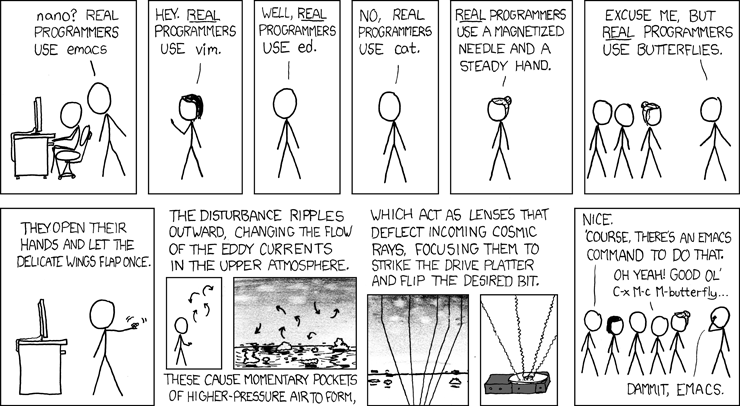
\includegraphics[width=\linewidth]{img/xkcd/real_programmers.png}
\caption*{{\small \textit{Real programmers set the universal constants at the start such that the universe evolves to contain the disk with the data they want. (xkcd.com/378)}}}
\end{figure}
